\documentclass[11pt]{article}
\usepackage{fullpage}
\usepackage{longtable}
\usepackage{graphicx}
\usepackage{amssymb,amsmath}
\usepackage{algorithm}
\usepackage{algpseudocode}
\usepackage{fancyvrb}
\usepackage{listings}
\usepackage{hyperref}
\usepackage{comment}
\usepackage{url}
\usepackage{authblk}
\begin{document}

\title{Extracting and Formatting Patent Data from USPTO XML}
\author{Gabe Fierro
    \thanks{gt.fierro@berkeley.edu}
}
\affil{Coleman Fung Institute for Engineering Leadership, UC Berkeley}
\date{\today}
\maketitle

\begin{abstract}
We describe data formatting problems that arise from extracting useful and
relevant data from the XML files distributed by USPTO. We then describe
solutions for a consistent data schematic that dictates in what format the
extracted data fields should be stored and how these transformations
should be applied to the data.
\end{abstract}

\section{Introduction}

The patent data available through the United States Patent and Trademark Office
(USPTO) is formatted as Extensible Markup Language (XML) and is an excellent
source of patent data, but is limited in its utility for statistical research
by a collection of idiosyncrasies that affect how the data may be understood.
An effective parser for this data must be made aware of such inconsistencies
and deficiencies so as to provide pristine and operable output.

The main goal of our parser is to create a cleaner, more modular solution to
the above problem. We want to make it easy to extract the data we want, and
facilitate further extensions on the parser so that we can apply it to new data
sources and adapt the output to new destinations. Furthermore, we want to
extract data in a consistent matter, agreeing upon standards regarding text
encodings, string formatting, order of tags, and other relevant issues.

A good parser will extract data in a form as close as possible to the original,
decreasing the chance that our process will add noise to the data. By
standardizing the process by which we extract relevant information from our raw
data, we can be more confident in the detail of that data. A high level of
detail is vital to the accuracy and effectiveness of the disambiguation
algorithm, which uniquely identifies inventors and is one of the primary
applications of the patent data.

\section{Parsing Toolchain and Data Process}

Considering the large volume of data we are addressing and the fact that new data
is available on a weekly basis, it is imperative to have a robust and pinelined
process for putting the data in a useable state.

We draw our raw patent data from three separate sources: the Harvard Dataverse
Network (DVN) collection of patent data from 1975 through 2010
~\cite{disambiguation}, the patent data used in the National Burearu of
Economic Research (NBER) 2001 study covering patent data from 1975 through 1999
~\cite{NBERw8498} and more recent patent grant data pulled from weekly
distributions of Google-hosted USPTO records ~\cite{googlefiles}. The DVN and
NBER data are available as SQLite databases, having already been catalogued.
The raw data we pull from Google arrives as concatenated XML files, and must be
parsed before it can be cleaned and enhanced with features such as geocoding
(associating latitude and longitude with assignees, inventors and the like).
For source URLs, please consult the appendix.

\begin{figure}[htb]
  \centering
  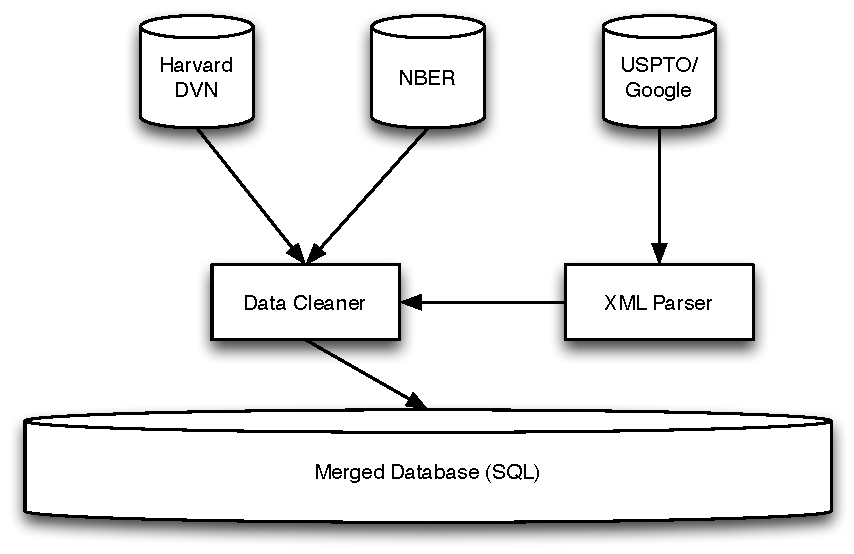
\includegraphics[width=.5\linewidth]{figs/parsing_toolchain}
  \caption{Basic view of data pipeline for processing patent data}
\end{figure}

After the raw XML has been parsed, the data is cleaned and enhanced and then
merged into the final database along with the NBER and DVN data.

\section{Text Format and Encoding}

Online distribution of data involves an awareness of the various datatypes used
to disseminate information, to wit, XML and HTML. In packaging data for such
distribution, resolution is usually sacrificed. Accents, brackets and other
extraordinary characters must be encoded or ``escaped'', sometimes in
non-obvious or non-standard ways.

\subsection{HTML Idioms and Escaping}

The downloaded patent data uses UTF-8 encoding and is packaged in valid XML
documents. There are several Document Type Definitions (DTDs) used by USPTO
that comprise the collections of XML documents we download, but it appears that
the most recent one has been used since about 2005. This means that when
dealing with recent data, the data formatting decisions outlined here will
apply to a large subset of the data we will be using. The fact that USPTO
distributes valid XML means that our parser can be built upon an easily
extensible base such as the Python 2.x \verb`xml.sax` module ~\cite{xmlsax},
which handles UTF-8 encoding and unescapes the following HTML entities:

\begin{figure}[htb]
  \begin{center}
\begin{tabular}{|l|c|r|}
  \hline
  Name & Character Literal & Escape Sequence \\
  \hline
  ampersand & ``\&'' & \texttt{\&\#x26;} \\
  emdash & ``---'' & \texttt{\&\#x2014;} \\
  left angle bracket & ``\textless{}'' & \texttt{\&lt;} \\
  right angle bracket & ``\textgreater{}'' & \texttt{\&rt;} \\
  \hline
\end{tabular}
\end{center}
\end{figure}

It is appropriate to keep all HTML escaped, but this can be easily
achieved through the escape method found in Python's built-in cgi
module.

An effort should be made to make the parsed text as human-readable as
possible while still maintaining the safety of escaped HTML, including
the translation of idioms such as
\texttt{<sub>\&\#x2014;</sub>}
(an underscore) to their character literals if doing so does not
conflict with the additional goal of HTML escaping, defaulting to the
Unicode encodings if we are unsuccessful.

\subsubsection{Takeaways}

We will use Python's \verb`cgi.escape` method ~\cite{cgiescape} to convert inner
tags (HTML tags that appear within the XML structure) to be HTML-safe. This
will help with distribution. We will also maintain UTF-8 text encoding by
normalizing the strings we extract from the XML documents by using Python's
\verb`unicodedata.normalize` method with the \verb`NFC` option
~\cite{unicodenormalize}.

\subsection{Escape Sequences}

Naive parsers will sometimes preserve the raw escape characters in the
outputted strings, e.g.  \verb`\r`,\verb`\n` and \verb`\t`.  These are not
essential to the semantic content of the tags we are extracting, especially
since the tags that do contain these escape sequences are not used in critical
applications such as the disambiguation.

Currently, the escape sequences only appear in the results from our original
production parser because the parser uses Python's builtin methods such as
\texttt{toxml()} and then removes tags using regular expressions. Resolving to
a standard of removing all escape sequences will help avoid confusion when
using string comparison to identify elements of patents, as most string
comparison engines take into account ``invisible'' characters such as escape
sequences.

\subsection{Combined Database Inconsistencies}

When combining the data from USPTO's XML repository with historical data from
DVN ~\cite{disambiguation} and data from the NBER ~\cite{NBERw8498}, a
surprising range of inconsistencies arises in regards to which ASCII sequences
are used to represent general patterns such as accents.

We have encountered the following inconsistencies across names alone:

\begin{enumerate}
    \item Missing accented letters: ``R\'{e}my'' becomes ``R my''
    \item Described accented letters: ``R\'{e}my'' becomes ``R acute over e my''
    \item Missing accents on accented letters: ``R\'{e}my'' becomes ``Remy''
    \item Correctly accented letters: ``R\'{e}my''
\end{enumerate}

The NBER data is consistent in dropping accents from the letters, and while
this is the most preferred of the 3 errors listed above, it is not optimal. It
is entirely possible to represent accented characters given the right ASCII
sequences, and an attempt should be made to standardize that. The preservation
of accents and other special ASCII characters is automatically handled by the
Python's \verb`unicodedata.normalize` method with the \verb`NFC` option.  By
normalizing to UTF-8, we can avoid the accent problems by keeping the accents.
This will require normalizing all of our historical data, as well as some more
intensive work on the NBER data.

Another inconsistency between the combined databases mentioned above is the
association of last name prefixes such as ``van der`` and ``de''. Because the
first names and last names of inventors are stored as separate columns in our
databases, which field these prefixes are associated with is vital to the
correctness and consistency of any future queries.

The NBER data is consistent in associating these prefixes with the beginning of
the last name, but the historical DVN data sometimes affiliates the prefixes
with the end of the first name.

The standard by which we will coerce our data is the association of such
prefixes with the beginning of the last name. This can be easily achieved by
splitting the first name field on spaces, and migrating all words after the
first to the last name field.

Relatedly, there are varying degrees of punctuation found in the combined
database.  Hyphens are often omitted from names, which is a design decision
incompatible with our desire to associate prefixes with the last name field;
replacing hyphens with spaces will turn names such as ``Sasson, Michael-David''
into ``David Sasson, Michael.'' Hyphens should be preserved to maintain
correctness. Other types of punctuation, e.g. periods and commas, can most
likely be ignored as they do not facilitate the specification of a given
individual.

\subsection{Document Numbers}

The easiest and most straightforward way to uniquely identify a given patent is
by its document number, which is a unique number assigned to applications that
have been issued patents. Document number comparisons are used for such
operations as counting up forward and backward citations. Obviously, a
consistent format for document numbers is imperative for any such operation on
the data. Because the combined database encompasses such a large range of
years, the data itself is nuanced by subtle changes in the various USPTO DTDs.
Document numbers may contain commas, character prefixes, or extraneous padding
0s. Indeed, our own database contains multiple versions of the same document
number. Inconsistencies arise between repositories of patents as well, making
it difficult to establish ground truths between disparate databases. The
USPTO's own website omits leading zeros and includes commas when displaying
numbers, but the downloaded XML files appear with leading zeros but without the
interspersed commas, e.g. ``123,456'' versus ``0123456''.

Non-utility patents have character prefixes that are useful for identifying the
type of document (see table). Fortunately, these prefixes are fairly consistent
across databases, and are easily removed for comparison with databases that do
not include the character prefixes.

\begin{figure}
  \begin{center}
\begin{tabular}{|l|r|}
  \hline
  D & Design patents \\
  PP & Plant patents \\
  R & Reissue patents \\
  T & Defensive publications \\
  H & SIR (Statutory Invention Registration) \\
  X & early X-patents \\
  \hline
\end{tabular}
\end{center}
\caption{Character prefixes for different document types ~\cite{patentprefixes}}
\end{figure}

To cut down search time, it would be ideal to avoid having to conduct a search
for both the padded and unpadded versions of a given patent number. This
presents us with two options: adding the leading 0 to all US patents, or
removing the leading 0.

In examining the databases, there are 70496082 patents with the leading 0, and
only 275554 without, at the time of writing. Adding a leading 0 to all patents
would solve the local consistency issue with a minimal amount of reprocessing
of the existing databases, but would fail to solve compatibility with other
repositories (that do not contain the leading 0) without additional
reprocessing of the entire database.

It makes more sense to remove the leading 0 from these patents; then, the
patent document numbers would be standardized without any superfluous bytes.
There is no obvious rationale for maintaining the leading 0, and eliminating it
would provide for easy cross-checking with external repositories. Though this
approach requires more reprocessing of the current data, this one-time cost is
worth the benefits.

\section{Acknowledgements}

We would like to thank the Fung Institute for Engineering Leadership for
supporting this research. This work is funded by the National Science
Foundation under grant 1064182.

{
\scriptsize
\bibliographystyle{acm}
\bibliography{manifesto}
}

\section*{Appendix: Data Sources and Code Repository}

\noindent The NBER data is available at \url{http://www.nber.org/patents/}.

\noindent The DVN data is available at \url{http://dvn.iq.harvard.edu/dvn/dv/patent/faces/study/StudyPage.xhtml;jsessionid=fd8595bd5c692dce0bef4ed95108?globalId=hdl:1902.1/15705&studyListingIndex=0_fd8595bd5c692dce0bef4ed95108}.

\noindent The USPTO data is available at \url{http://www.google.com/googlebooks/uspto-patents-grants-text.html}.

\noindent The parsing code and the patent processor toolchain can be found on Github at \url{https://github.com/funginstitute/patentprocessor/}.

\noindent Links to our merged database can be found at \url{https://github.com/funginstitute/downloads}.

\end{document}
